A \emph{concurrent datatype} is a datatype, for example, a queue, stack, set
or mapping, that can be safely accessed concurrently by multiple threads.
Operation invocations should appear to take place in a one-at-a-time order,
without interference.

Threads that use the concurrent datatype can act much as they would with a
sequential datatype: the implementer of the threads does not need to think
much about concurrency.  

The implementer of the concurrent datatype \emph{does} have to think about
concurrency, and ensure different operation calls do not interfere with one
another.  But that concurrency is local, often inside a single object: local
reasoning is much easier than global reasoning.  And there's a lot of scope
for re-using concurrent datatypes.

Datatype-based concurrent programming encapsulates \emph{all} the concurrency
within a small number of concurrent datatypes.

%%%%%%%%%%%%%%%%%%%%%%%%%%%%%%%%%%%%%%%%%%%%%%%%%%%%%%%%%%%%

\section{Example: a concurrent queue}

To illustrate some of the ideas, we will implement a concurrent queue.  First,
we should ask: what interface should a concurrent queue have?  A sequential
queue would typically have an interface like:
%
\begin{mysamepage}
\begin{scala}
trait Queue[T]{
  /** Enqueue x. */
  def enqueue(x: T): Unit

  /** Dequeue a value.  Precondition: the queue is not empty. */
  def dequeue(): T

  /** Is the queue empty? */
  def isEmpty: Boolean
}
\end{scala}
\end{mysamepage}
%
The |dequeue| operation has a non-trivial precondition, so client code that
uses the queue would be expected to check this first, for example, via code
such as:
\begin{scala}
  if(queue.isEmpty){ ... /* Handle the empty queue. */ } 
  else{ val x = queue.dequeue(); ... /* Do something with £x£. */ }
\end{scala}

However, this won't work with multi-threaded code: thread~$t$ might check that
the queue is non-empty; but then other threads might empty the queue before
$t$ attempts the |dequeue|, at which point the precondition is violated.  This
is a time-of-check to time-of-use (TOCTTOU) problem: there is a delay between
the thread checking the relevant precondition and performing the operation that
depends upon it, during  which the precondition becomes false; several
exercises in Chapter~\ref{chap:intro} considered the same issue.

We saw in Chapter~\ref{chap:clientServer} that there are two main ways of
dealing with operations that have a non-trivial precondition.  One way is to
return a special value to indicate that the precondition does not hold.  In
Scala, it is natural to use an |Option| value, with |None| indicating that the
precondition does not hold.  In some circumstances, it might be appropriate
(and more efficient) to use |null| for this, if |null| can never be returned
when the precondition does hold.  An alternative, is for the operation to
throw an exception, and expect the thread to catch it.  Operations that treat
preconditions in this way are called \emph{total}: they can take effect in any
state.

The other way to deal with the case that the precondition does not hold is to
block the thread until the precondition becomes true.  Such operations are
called \emph{partial}.

We will start with a total concurrent queue, with the following interface,
where the |dequeue| operation returns an |Option| type, with |None| used to
indicate am empty queue. 
%
\begin{mysamepage}
\begin{scala}
/** A total queue. */
trait TotalQueue[T]{
  /** Enqueue x. */
  def enqueue(x: T): Unit

  /** Dequeue a value.  Returns £None£ if the queue is empty. */
  def dequeue(): Option[T]

  /** Shut down the queue. */
  def shutdown: Unit
}
\end{scala}
\end{mysamepage}

A thread that performs a |dequeue| should handle both cases, for example, via
code such as:
\begin{scala}
  queue.dequeue() match{
    case Some(x) => ... // Do something with £x£.
    case None => ... // Handle the empty queue.
  }
\end{scala}

Figure~\ref{fig:total-queue-server} gives a straightforward implementation of
a total queue that encapsulates a server.  But we could also implement the
queue using one of the techniques we'll see later in the course.  The server
stores the queue itself (using a |Queue| from the Scala API).  Clients use
channels to cause the server to enqueue and dequeue values.  Note that the
server handles operations in a one-at-a-time way, preventing operations from
interfering with one another.  We also include a |shutdown| operation, to
provide a way to terminate the server thread, and so allow garbage collection.

%%%%%

\begin{figure}
\begin{scala}
class ServerTotalQueue[T] extends TotalQueue[T]{
  // Channels used for enqueueing and dequeueing.
  private val enqueueChan = new SyncChan[T]
  private val dequeueChan = new SyncChan[Option[T]]

  def enqueue(x: T) = enqueueChan!x

  def dequeue(): Option[T] = dequeueChan?()

  private def server = thread("ServerTotalQueue"){
    val queue = new scala.collection.mutable.Queue[T]
    serve(
      enqueueChan =?=> { x => queue.enqueue(x) }
      | dequeueChan =!=> { 
          if(queue.nonEmpty) Some(queue.dequeue()) else None 
        }
    )
  }

  fork(server)

  def shutdown() = { enqueueChan.close; dequeueChan.close }
\end{scala}
\caption{A total queue implemented using a server.}
\label{fig:total-queue-server}
\end{figure}

%%%%%

\begin{instruction}
Study the details of the implementation.
\end{instruction}

%%%%%

\section{Correctness}

We want to test the concurrent total queue implementation.  But first, we need
to understand better what ``correct'' actually means in this case.  And, by
extension, we will understand correctness conditions for other concurrent
datatypes. 

Informally, the correctness condition is:
%
\begin{itemize}
\item Operation invocations should take place (apparently) in a one-at-a-time
  way, without interference between invocations.

\item The point at which each invocation takes effect is between the time the
invocation was invoked and when it returns.  

\item The values returned by invocations should be the same as for a sequential
queue (when the invocations are performed in the same order). 
\end{itemize}
%
The correctness condition for other concurrent datatypes is the same, except
with the sequential queue in the third item replaced by a corresponding
sequential datatype.

This property is called \emph{linearization}.  The points at which invocations
appear to take effect are called \emph{linearization points}.  It is an
attractive property, because it matches most programmers' mental models of how
such a concurrent datatype should behave. 

We will give a more formal definition of linearization shortly.  But first, we
give some examples.  

Figure~\ref{fig:linearization} gives four timelines.  In each, time goes from
left to right.  Each row is labelled with the identity of a thread
(e.g.~$t_0$).  Each horizontal line represents the execution of an operation,
with the endpoints of the line representing the call of the operation and its
return, respectively; the line is labelled with the name of the operation, its
parameters, and the value returned, although we omit the latter for
operations, like |enqueue|, that return the trivial |Unit| type.

%%%%%

%\unScalaMid
\begin{figure}
\def\X{node{\scalastyle X};}
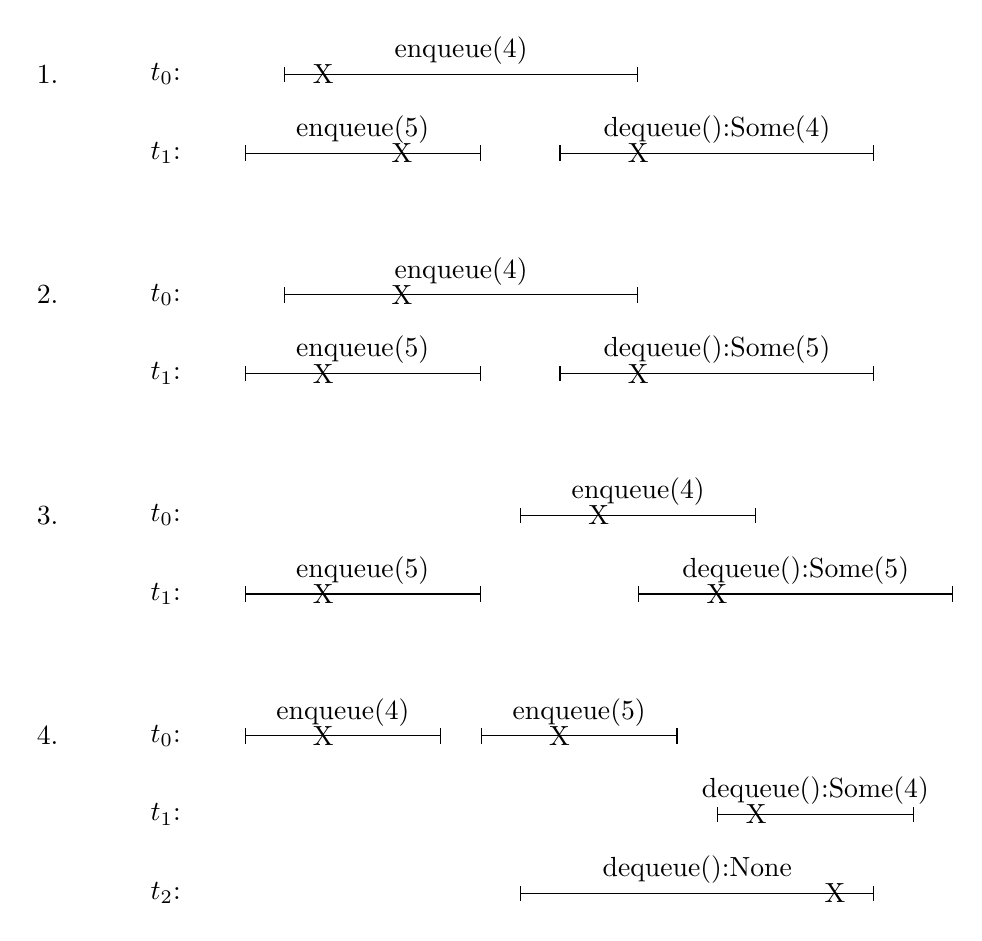
\begin{tikzpicture}[scale=1.0]
\draw (-1.5,0) node{1.};
\draw (0,0) node {$t_0$:}; 
\draw[|-|] (1.5,0) -- node[above] {\scalashape enqueue(4)} (6,0);
\draw(2,0) \X;
\draw (0,-1) node {$t_1$:}; 
\draw[|-|] (1,-1) -- node[above] {\scalashape enqueue(5)} (4,-1);
\draw(3,-1) \X;
\draw[|-|] (5,-1) -- node[above] {\scalashape dequeue():Some(4)} (9,-1);
\draw(6,-1) \X;
%%%%%
\draw (0,-2.8) node (O) {$t_0$:}; 
\draw (O)++(-1.5,0) node{2.};
\draw[|-|] (O)++(1.5,0) -- node[above] {\scalashape enqueue(4)} ++(4.5,0);
\draw (O)++(3,0) \X;
\draw (O)++(0,-1) node {$t_1$:}; 
\draw[|-|] (O)++(1,-1) -- node[above] {\scalashape enqueue(5)} ++(3,0);
\draw (O)++(2,-1) \X;
\draw[|-|] (O)++(5,-1) -- node[above] {\scalashape dequeue():Some(5)} ++(4,0);
\draw(O)++(6,-1) \X;
%%%%%
\draw (O)++(0,-2.8) node (O) {$t_0$:}; 
\draw (O)++(-1.5,0) node{3.};
\draw[|-|] (O)++(4.5,0) -- node[above] {\scalashape enqueue(4)} ++(3,0);
\draw (O)++(5.5,0) \X;
\draw (O)++(0,-1) node {$t_1$:}; 
\draw[|-|] (O)++(1,-1) -- node[above] {\scalashape enqueue(5)} ++(3,0);
\draw (O)++(2,-1) \X;
\draw[|-|] (O)++(6,-1) -- node[above] {\scalashape dequeue():Some(5)} ++(4,0);
\draw (O)++(7,-1) \X;
%%%%%
\draw (O)++(0,-2.8) node (O) {$t_0$:}; 
\draw (O)++(-1.5,0) node{4.};
\draw[|-|] (O)++(1,0) -- node[above] {\scalashape enqueue(4)} ++(2.5,0);
\draw (O)++(2,0) \X;
\draw[|-|] (O)++(4,0) -- node[above] {\scalashape enqueue(5)} ++(2.5,0);
\draw (O)++(5,0) \X;
\draw (O)++(0,-1) node{$t_1$:};
\draw[|-|] (O)++(7,-1) -- 
  node[above] {\scalashape dequeue():Some(4)} ++(2.5,0);
\draw (O)++(7.5,-1) \X;
\draw (O)++(0,-2) node{$t_2$:};
\draw[|-|] (O)++(4.5,-2) -- 
  node[above] {\scalashape dequeue():None} ++(4.5,0);
\draw (O)++(8.5,-2) \X;
\end{tikzpicture}
\caption{Four timelines illustrating linearization.}
\label{fig:linearization}
\end{figure}
%\scalaMid

%%%%%

In timeline~1, thread $t_0$ enqueues~|4|, and thread $t_1$ enqueues~|5| and
dequeues~|4| (so the |dequeue| operation returns |Some(4)|).   This history is
linearizable, if the operations take place at the points
labelled~``{\scalashape X}''.  This would correspond to a sequential
history:\footnote{We denote sequences within angle brackets, $\seq{\ldots}$.}
\[
\seq{ \sm{enqueue(4)},\, \sm{enqueue(5)},\, \sm{dequeue():Some(4)}}
\]
which would be valid on a corresponding sequential queue.

%%%%%

Timeline~2 is similar, except the |dequeue| returns |Some(5)|.  This is also
linearizable, where the operations take place at the points
labelled~``{\scalashape X}'', which would correspond to the valid sequential history
\[
\seq{ \sm{enqueue(5)},\, \sm{enqueue(4)},\, \sm{dequeue():Some(5)}}
\]

%%%%%

%\begin{slide}
\heading{Linearization examples - 3}

With the following timeline, the dequeue must return 5: any other return would
not be linearizable.
%
%% \begin{tikzpicture}[scale=0.8]
%% \draw (0,0) node {$t_0$:}; 
%% \draw[|-|] (4.5,0) -- node[above] {\scalashape enqueue(4)} (7.5,0);
%% %\draw(3,0) node{X};
%% \draw (0,-1) node {$t_1$:}; 
%% \draw[|-|] (1,-1) -- node[above] {\scalashape enqueue(5)} (4,-1);
%% %\draw(2,-1) node{X};
%% \draw[|-|] (6,-1) -- node[above] {\scalashape dequeue(): Some(5)} (10,-1);
%% %\draw(6,-1) node{X};
%% \end{tikzpicture}

Example 4

%% And the following history is not linearizable, because the queue is non-empty
%% throughout $t_2$'s operation.
%% %
%% \begin{tikzpicture}[scale=0.8]
%% \draw (0,0) node {$t_0$:}; 
%% \draw[|-|] (1,0) -- node[above] {\scalashape enqueue(4)} (3.5,0);
%% \draw[|-|] (4,0) -- node[above] {\scalashape enqueue(5)} (6.5,0);
%% \draw (0,-1) node{$t_1$:};
%% \draw[|-|] (7,-1) -- node[above] {\scalashape dequeue():Some(4)} (9.5,-1);
%% \draw (0,-2) node{$t_2$:};
%% \draw[|-|] (4.5,-2) -- node[above] {\scalashape dequeue():None} (9,-2);
%% \end{tikzpicture}
%% \scalaMid
%% \end{slide}

%%%%%


\framebox{Formal definition of linearization.}

%%%%%

\begin{slide}
\heading{Synchronous channels}

It is important that we use \emph{synchronous channels} in the server-based
queue.  Suppose we used buffered channels.  Then the following behaviour is
possible.
%
\begin{enumerate}
\item Thread $t_1$ calls |enqueue(5)|, but the value~|5| stays in the
  |enqueueChan|, even after $t_1$ returns;

\item Thread $t_2$ calls |dequeue()|, and the server sends it |None|.
\end{enumerate}

Alternatively
%
\begin{enumerate}
\item The server sends |None| on |dequeueChan|, and that value stays in the
  channel; 

\item Thread $t_1$ calls |enqueue(5)|, and this value is received and stored
  by the server; 

\item Thread $t_2$ calls |dequeue()|, and receives the |None| sent earlier.
\end{enumerate}
\end{slide}

%%%%%

\begin{slide}
\heading{Synchronous channels}

Using synchronous channels, the invocations have an effect in the order of the
channel communications.  This order is compatible with the order of the
invocations calls and returns.

We will always use synchronous channels when implementing a concurrent
datatype using a server thread.   
\end{slide}


%%%%%

\begin{slide}
\heading{Testing for linearizability}

How can we test for linearizability?

Basic idea: 
%
\begin{itemize}
\item Run some threads on the concurrent queue, performing random |enqueue|
and |dequeue| operations, and record the history of operation calls and
returns;

\item Search for a corresponding sequential history that explains
linearizability, and that is a valid history for the corresponding sequential
datatype.  If none is found, signal an error.
\end{itemize}
%
Repeat many times.
\end{slide}

%%%%%

\begin{slide}
\heading{Testing for linearizability}

I've developed a framework to support such testing\footnote{{Testing
    for Linearizability}, Gavin Lowe, \textit{Concurrency and Computation},
    Practice and Experience, 29 (4), 2017,
  \url{http://www.cs.ox.ac.uk/people/gavin.lowe/LinearizabiltyTesting/}.},
and, in particular, investigated algorithms for testing whether a concurrent
history is linearizable.

In the next slides, we'll see a stripped-down testing script that uses this
(the full version can be used with multiple concurrent queue implementations,
and replaces the numerical constants by variables, specifiable via the command
line).

\vfill
\end{slide}

%%%%%

\begin{slide}
\heading{A small testing script}

The test program works on a concurrent datatype of some type~|C|; here we use
a |TotalQueue| containing |Int|s.  The test program
also requires a corresponding, \emph{immutable, deterministic}
sequential specification datatype~|S|, here an immutable queue from the Scala
API.
%
\begin{scala}
object QueueTest{
  type C = TotalQueue[Int]
  type S = scala.collection.immutable.Queue[Int]
  ...
}
\end{scala}
\end{slide}

%%%%%

\begin{slide}
\heading{A small testing script}

For each operation |op : A| on the concurrent datatype, we need a
corresponding function |seqOp : S => (A, S)| on the sequential datatype, which
returns the same value as the concurrent operation\footnote{More precisely,
  the two values should be equal, as tested using the ``{\scalashape ==}''
  method.}, paired with the new value of the sequential datatype.  These are
normally simple wrappers around API code.
%
\begin{scala}
  def seqEnqueue(x: Int)(q: S) : (Unit, S) = ((), q.enqueue(x))
  def seqDequeue(q: S) : (Option[Int], S) =   
    if(q.isEmpty) (None, q) 
    else{ val (r,q1) = q.dequeue(); (Some(r), q1) }
\end{scala}
\vfill
\end{slide}

%%%%%

\begin{slide}
\heading{A small testing script}

The main part of the test program is the definition of a |worker| function
that performs and logs operations on the concurrent datatype, associating each
concurrent operation with a corresponding operation on the sequential
datatype.  Here, the worker performs 200 operations; each is (with probability
0.3) an enqueue of a random value, or (with probability~0.7) a dequeue.
\begin{scala}
  def worker(me: Int, log: LinearizabilityLog[S, C]) = {
    val random = new scala.util.Random
    for(i <- 0 until 200)
      if(random.nextFloat <= 0.3){
        val x = random.nextInt(20)
        log(_.enqueue(x), s"enqueue($x)", seqEnqueue(x))
      }
      else log(_.dequeue(), "dequeue()", seqDequeue)
  }
\end{scala}
\end{slide}

%%%%%

\begin{slide}
\heading{A small testing script}

The worker takes a log object |log| as a parameter; each operation is
performed and logged via a call to |log|, taking three parameters:
%
\begin{itemize}
% \item
% The identity of the thread doing the operation;

\item
The operation to be performed on the concurrent datatype;

\item A string describing the operation (this is used in debugging output in
the case that a non-linearizable history is found, and is also used internally
for optimisations; semantically different operations should have different
strings);

\item
The corresponding operation on the sequential datatype.
\end{itemize}

The call to |log| logs the invocation of the concurrent operation,
performs the concurrent operation, and logs the result returned.
\end{slide}
\begin{slide}
\heading{A small testing script}

The main test for linearizability is performed at line~\ref{line:maintest},
below, repeated so as to consider 1000 histories.  The  tester
takes as arguments: the sequential datatype; the concurrent datatype; the
number |p| of worker threads to run; and the definition of a worker thread.
%
\begin{scala}[numbers=left,numberstyle=\scriptsize]
  def main(args: Array[String]) = for(i <- 0 until 1000){
    val concQueue = new ServerTotalQueue[Int] // The concurrent queue
    val seqQueue = Queue[Int]() // The sequential specification queue
    val tester = LinearizabilityTester[S, C](seqQueue, concQueue, 4, worker _)
    assert(tester() > 0)£\label{line:maintest}£
  }
\end{scala}
%
The linearizability tester runs |p| workers concurrently, logging the
operation calls on the concurrent datatype.  It then tests whether the
resulting history is linearizable, returning a positive result if so.
\end{slide}

%%%%%

\begin{slide}
\heading{Controlling the search space}

The algorithm for testing linearizabilty, in effect, considers all possible
linearizations of the history, i.e.~all ways of ordering the operations
consistent with the history.  It then tests whether that ordering is
compatible with the sequential datatype, i.e.~whether performing the
corresponding sequential operations in the same order would give the same
results. 

Thus the algorithm considers all  states that the sequential
specification object could get into after a prefix of such linearizations.
%
If there are too many such states, this will take a long time.  It's therefore
a good idea to design the test so that such bad cases are very unlikely.
\end{slide}

%%%%%

\begin{slide}
\heading{Controlling the search space}

With a queue, the linearizability tester considers all possible states of the
sequential queue formed by permuting concurrent enqueue operations.  This
number grows exponentially with the length of the queue.  We therefore try to
avoid the length of the queue growing too much.  We did this in the earlier
testing harness by making dequeues more frequent than enqueues.
\end{slide}

%%%%%

\begin{slide}
\heading{Logging}

By default, the linearizability tester logs operation calls and returns using
thread-local logs, pairing each event with a timestamp.  We saw a similar
technique in an earlier chapter.  If you're using an operating system that
doesn't support timestamps property, setting the optional parameter |tsLog| to
|false| will use a different type of log.
%
\begin{scala}
  val tester = LinearizabilityTester[S, C](
    seqQueue, concQueue, 4, worker _, £\scalastyle\color{red} tsLog = false£)
\end{scala}
\end{slide}

%%%%%

%% \begin{slide}
%% \heading{Exercise}

%% Implement and test a total concurrent stack using similar techniques.
%% \end{slide}
